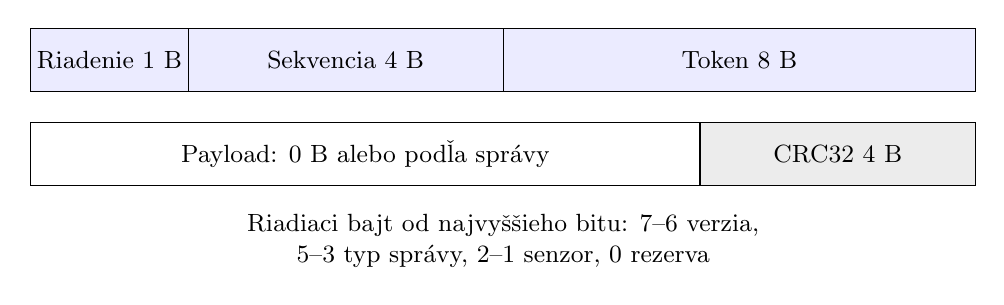
\begin{tikzpicture}[x=1cm,y=1cm,font=\small]
\draw[fill=blue!8] (0,0) rectangle (2,0.8);
\draw[fill=blue!8] (2,0) rectangle (6,0.8);
\draw[fill=blue!8] (6,0) rectangle (12,0.8);
\node at (1,0.4) {Riadenie 1 B};
\node at (4,0.4) {Sekvencia 4 B};
\node at (9,0.4) {Token 8 B};
\draw (0,-1.2) rectangle (8.5,-0.4);
\draw[fill=gray!15] (8.5,-1.2) rectangle (12,-0.4);
\node at (4.25,-0.8) {Payload: 0 B alebo podľa správy};
\node at (10.25,-0.8) {CRC32 4 B};
\node[align=center] at (6,-1.9) {Riadiaci bajt od najvyššieho bitu: 7--6 verzia,\\5--3 typ správy, 2--1 senzor, 0 rezerva};
\end{tikzpicture}
